% Template for ICASSP-2016 paper; to be used with:
%          spconf.sty  - ICASSP/ICIP LaTeX style file, and
%          IEEEbib.bst - IEEE bibliography style file.
% --------------------------------------------------------------------------
\documentclass{article}
\usepackage{spconf,amsmath,graphicx,float}

% Example definitions.
% --------------------
\def\x{{\mathbf x}}
\def\L{{\cal L}}

% Title.
% ------
\title{Automated Landmark Recognition Powered by Deep Learning}
%
% Single address.
% ---------------
\name{Jifu Zhao}
\address{Department of Nuclear, Plasma, and Radiological Engineering \\
University of Illinois at Urbana-Champaign, Urbana, Illinois 61801, USA}

\begin{document}
%\ninept
%
\maketitle

\section{Introduction}
\label{sec:intro}
With the development of deep learning techniques, especially convolutional neural networks (CNN), we have achieved huge breakthrough in computer vision. On ImageNet Large Scale Visual Recognition Challenge, computer have already achieved human-level error rate. Some classical CNN models, such as VGG, ResNet, Inception and so on, have been widely adapted to various computer vision tasks. 

One important factor that contributes to the success of image object recognition is the large number of training images. For example, CIFAR-10 dataset contains of 60,000 color images in 10 classes, with 6,000 images per class, and ImageNet dataset contains of 1,000 objects. In addition to similar problems with large amount of training images, there are problems without large amount of training set or the number of objects is too large such that some objects only have a small number of or even one images in training set, which make it impossible to apply the same supervised algorithms. Problems like face recognition, landmark recognition and so on, is very challenging due to small number of training images for each object.

This work, using a recently released landmark dataset from Google, try to explore the application of deep learning methods on landmark recognition problems.

\section{Problems}
\label{sec:problem}



\section{Dataset}
\label{sec:dataset}



\section{Conclusion}
\label{sec:conclusion}


%\begin{figure}[htbp]
%\centering
%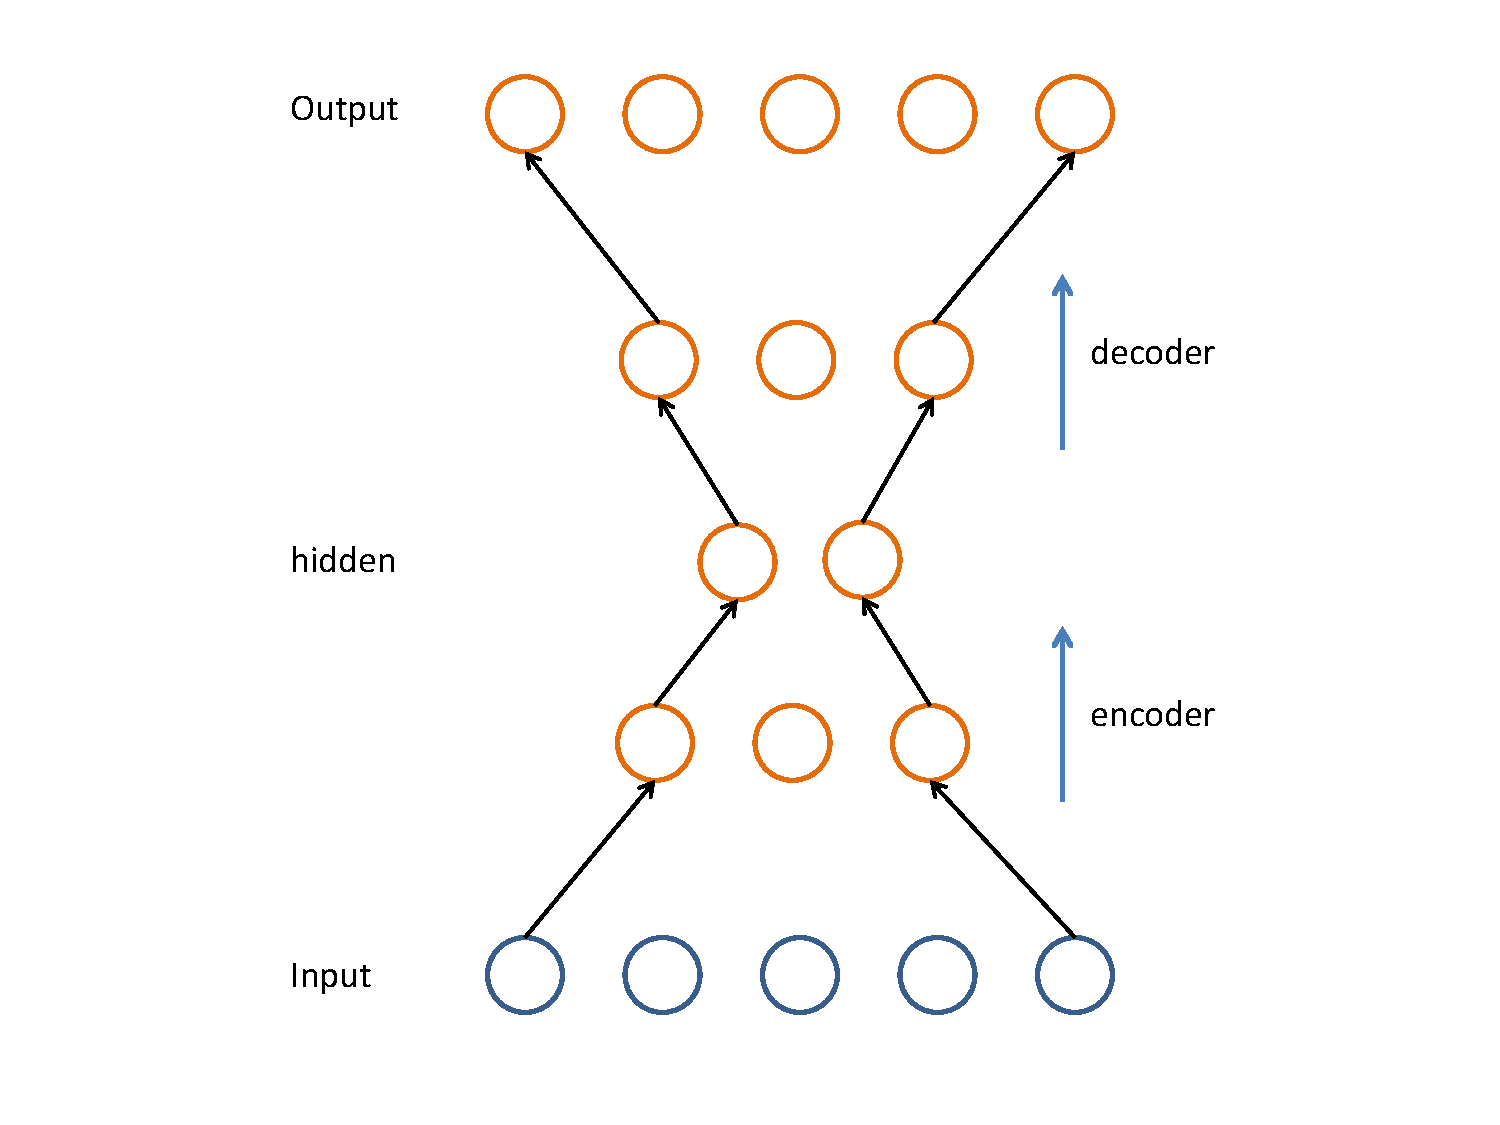
\includegraphics[width=8.5cm]{./figures/autoencoder.pdf}
%\caption{Illustration of auto-encoder system.}
%\label{fig:autoencoder}
%\end{figure}

\vfill\pagebreak

% References should be produced using the bibtex program from suitable
% BiBTeX files (here: strings, refs, manuals). The IEEEbib.bst bibliography
% style file from IEEE produces unsorted bibliography list.
% -------------------------------------------------------------------------
\bibliographystyle{IEEEbib}
%\bibliography{strings,refs}
\bibliography{strings}

\end{document}
